\documentclass[11pt]{article}
\usepackage[T1]{fontenc}
\usepackage[latin1]{inputenc}
\usepackage{enumerate}
\usepackage{setspace}
\usepackage{amsmath,amssymb,amsthm}
\usepackage{graphicx}
\usepackage{bbm}
\usepackage[round]{natbib}
\usepackage[nohead]{geometry}
\usepackage[bottom]{footmisc}
\usepackage{indentfirst}
\usepackage{endnotes}
\usepackage{graphicx}%
\usepackage{eurosym}
\usepackage{array}
\usepackage{booktabs}
\usepackage{subcaption}
\usepackage{hyperref}
\usepackage[capposition=top]{floatrow}
\renewcommand{\labelitemi}{--}
\renewcommand{\labelitemii}{$\bullet$}
\bibliographystyle{chicago}
% \geometry{left=1in,right=1in,top=1.00in,bottom=1.0in}
\let\olditemize\itemize
\renewcommand{\itemize}{
  \olditemize
  \setlength{\itemsep}{-1pt}
}

\begin{document}

\title{Price dispersion on the French retail gasoline market\ \\ \ \\(Very preliminary)}
\author{Etienne Chamayou\thanks{e-mail:
\textit{etienne.chamayou@ensae.fr}}\medskip\\{\normalsize CREST and Department of Economics, Ecole Polytechnique}}
\maketitle

\sloppy%

\onehalfspacing

\textbf{Abstract:}
Abstract to be added here.

\strut

\textbf{Keywords:} Industrial Organization, Search

\strut

\textbf{JEL Classification Numbers:} XXX

\pagebreak%
\doublespacing

\section{Abstract}
\setcounter{page}{1}

This article studies price dispersion on the French retail gasoline market, following and discussing the methodology employed by \cite{TAP11} with US data to test a standard prediction of consumer search models: randomized pricing. Even though the presence of differentiation and shocks affecting competition in French data are shown to require careful treatment, findings are consistent with \cite{TAP11}. Price rankings in local markets exhibit significant variability over time, with variability increasing in distance between stations. This arguably supports the connection made by \cite{STI61} between price dispersion and the "ignorance in the market". Price dispersion furthermore decreases with cost and increases with the number of firms, in accordance with predictions from a model a la \cite{VAR80}.

\section{Introduction}

The seminal paper of the consumer search literature, \cite{STI61}, advocated the idea that a key element of competition was the relation between the cost of searching for prices by consumers and price dispersion i.e. the lasting existence of different prices for a homogeneous product. While the paper only provides evidence of static price dispersion (e.g. retailers posting different prices for a given car model in a suburb), thus leaving open discussions about differentiation, the empirical literature would soon strive to make the case stronger by considering temporal price dispersion, namely sellers'price moving within the market distribution over time. This was long done essentially by considering panel data of standard goods sold at various stores, introducing fixed effects to account for potential differentiation, and producing statistics to account for changes of rank in the distribution of prices (e.g. quantile to quantile changes). Shortcomings typically included the fact that price distributions included sellers that were not necessarily operating in the same environment.

As argued by \cite{TAP11}, the retail gasoline market appears to be particularly relevant to a discussion about the role of consumer search. The presence of sustained retail price variations due to oil cost fluctuations generates an information issue that consumers cannot ignore. High product homogeneity offers the opportunity to work with raw prices rather than prices which may have been cleaned inadequately. And most importantly, current data allow to compare prices posted by sellers which are actually competing within the same market.

Competition in the retail gasoline market has attracted a lot of attention in France over last years. In 2006, a governmental website was launched by the Ministry of Economics with a view to increase transparency in the market. All stations having sold over 500m3 of gasoline over the previous year are since then required to keep prices posted on the website. In 2011, a large inquiry was ordered by the government as retail price adjustments to oil cost variations were suspected to be faster upwards than downwards (the "Rocket and feathers" hypothesis first investigated by \cite{BAC91} in the UK). Little evidence was yet found and the report rather emphasized signs pointing toward a significant degree of competitiveness. Finally, in August 2013, following an election promise, the governement of the then newly elected French President Fran�ois Hollande has implemented a 3c/l tax cut for 3 month, asking gasoline retailers on the market to produce the same effort.

The effect of the creation of the website has not been evaluated, probably for lack of data before 2006. The 2011 report yet called for further development of the website, and Germany has taken a similar initiative in 2012. More generally, in a context where dynamic prices generate heightened debates (e.g. Amazon), the idea to monitor competition by constraining firms to increase transparency enjoys strong popularity among politicians. The theory of consumer search however tells us that measures affecting information are far from innocuous. On the one hand, in a situation of strong competition, aligned prices provide little incentive for consumers to search, thus undermining the stability of such an equilibrium. Contrarily, collusion appears quite sustainable in a context where a reliable website makes monitoring costless and, again, aligned prices discourage search by consumers.

TODO: contribute to the understanding of the relation between dispersion and search, taking advantage of the heterogeneity in local contexts of competition.

\section{Literature}

Whereas price dispersion had already been obtained in some settings, \cite{VAR80} innovated by modeling price dispersion as a result of mixed pricing strategies. According to the paper, price dispersion thereby obtained could be interpreted as "temporal" price dispersion, typically in the form of "sales". This provided a rationale for rank reversals i.e. competing sellers being successively cheaper/more expensive one vs. another.

The dynamic interpretation of the model is not unambiguous however. In the model, firms are ex-ante indifferent between all prices in the support of the equilibrium price distribution (also holds in terms of randomization over utilities). Ex-post, indifference obviously no more exists. The cheapest firm attracts shoppers but would be better off increasing its price to match the second cheapest price. Other firms may consider either increasing price to consumers' reservation price, or trying to undercut the cheapest firm. Consequently, price rigidity should lead to carefully interpret results regarding rank reversals.

\cite{TAP11} take advantage of a data set including daily prices of gas stations in the US over one year and a half. \cite{TAP11} argue that gas stations located across the same corner should display less rank reversal vs. those a bit further as consumers' information on prices should decrease with distance. This is shown to be true (use of the Kolmogorov-Smirnov test to prove that rank reversals are drawn from different distributions for gas stations respectively 1-mile and 2-mile away from each other and of quantile regressions of each pair of stations' standard deviation on distance between stations) and all the more convincing as close gas stations display a lower average spread. Regressions of price dispersion (measured in the various ways described previously) on marginal costs and the number of firms in the market within 1-mile yields results consistent with the extension of \cite{VAR80} proposed by the paper (resp. negative and positive impacts).

\section{The French retail gasoline market}

\subsection{Information source overview}

As is put by the 2011 governmental report on the French retail gasoline market, "nobody knows precisely the number of gas stations operating in the markets". As a consequence, all efforts to investigate competition in the French retail gasoline market start with a difficult quest for trustworthy information. The following section offers a brief overview of the information sources and their limits.

Two websites relying on crowdsourcing i.e information provided by users, Carbeo and Zagaz, were launched respectively in 2005 and 2006. In 2007, a law/decree was published making it mandatory for gas stations having sold over 500m$^{3}$ gas the previous year to keep prices posted on the governmental website prix-carburants.economie.gouv.fr. The 2011 governmental report notes that shortly after its launch the website started being scraped in a signficant way, to the extent that user experience was deteriorated. In 2009, as a consequence, licenses were created to allow for resale of price data for internal or commercial use.

The launch of the governemental website exercised significant pressure on the young websites Zagaz and Carbeo. Zagaz still exists and has stuck to its pure crodwsourcing philosophy. Carbeo, on the contrary, purchased a licence from the governement as early as 2009. Interestingly, in 2011, the governemental body in charge of town and country planning worked with Zagaz data to study the French retail gas station network. Zagaz most likely remains the most comprehensive source of information but suffers from a lack of users in many regions.

\subsection{Retail gasoline distribution}

The size of the French gas station network has been decreasing at a steady pace over the last decades, from c. 40,000 in 1980 to c. 12,000 currently, mainly as a result of increased car capacities.  A strong competitive pressure has furthermore been generated by supermarkets progressively penetrating the market. They currently represent c. 50\% of sales in retail gasoline.

The exact number of gas stations operating in the market is uknown. As of May 20, 2014, Zagaz lists c. 12,832 gas stations, but no price was recorded over the last months/years for many of them so that this figure most certainly overestimates the actual number of gas stations. In April 2013, UFIP quoted the number of 11,476 (4,979 supermarkets and 6,497 "traditional" players, source: Nielsen).

Gas stations are essentially either owned and operated by a chain or with a "location-gerance" contract according to which the manager receives a commission on gasoline sold (e.g. only 200 gas stations set prices independently among gas stations from Total brand). There is significant evidence that many gas stations hardly make any profits: oil companies exiting the market (Shell, BP), drastically reducing the size of their organic network (Esso), bankrupts or terminations of independent gas stations etc.

Key cost components are the cost of wholesale gasoline, including delivery fees,  gas station operating expenses, and taxes. Taxes included a fix part called TICPE, which slightly varies between regions, and the standard variable VAT (19.6\% over the period studied, which bear on cost and TICPE).
 
\subsection{Demand}

Diesel consumption currenlty accounts for c. 80\% of total gasoline consumption. This evolution was achieved through a lower tax on diesel. At a very aggregate level, two kinds of consumers can be distinguished: businesses and individual customers. Businesses are typically offered card programs which allow them to monitor employees' consumptions and obtain rebates. An important implication is that the price of the gas station is irrelevant (or only partly relevant) to a signicant number of transations in the market.
Consumer can get information about prices from a variety of sources: at gas stations, on gps, on mobile phone applications (e.g. Zagaz, Carbeo, Essence Free) and on a computer or mobile phone browser (Prix-Carburants.gouv.fr).

\section{Data}

\subsection{Data overview}

Data about daily diesel prices, gas station locations, opening hours and amenities were collected from website prix-carburants.gouv.fr. Gas station location was verified and improved with data from Zagaz (information provided by users about gas station locations was observed to be of better quality). Finally, the gas station database was merged with INSEE data in order to add information about local markets (rural/center/suburb, population etc.). Rotterdam wholesale diesel price is used as proxy for gas stations' variable costs.

\subsection{Context of studied period}

The period covered is marked by two significant events of different natures. One is a change of pricing strategy by a leading retail brand affecting the whole country and the other is a governmental intervention.

The first event is the progressive conversion by the historical incumbent "Total" of a number of its gas stations to low cost gas stations branded "Total Access" i.e. gas stations whose prices are aligned with supermarket gas stations. The French retail gasoline market is indeed characterized by the penetration of supermarkets, which currently account for over 50\% of total sales. Though these conversions are obviously not heterogeneous shocks to the market, they yet involve a significant number of gas stations lowering their price by c. 0.10 \euro per liter virtually overnight.

The second event is of political nature.
On August 29, 2012, a decrease in price of 6c per litre was announced by the government, following an election promise made by Francois Hollande. This decrease was (to be) achieved by a decrease of tax of 3c per litre and an equivalent "effort" by gas station operators. Also, it must be noted that a small portion of the tax on gasoline is set by regions on an annual basis.

\subsection{Descriptive statistics}

\textbf{Retail price vs. wholesale cost of diesel}

Descriptive statistics are provided for a period of 640 days starting September 9, 2011 and ending May 6, 2013. Four subperiods of data are missing whose respective day lengths are 11 (2012/07/08-2012/07/18), 10 (2012/08/13-2012/08/22), 49 (2012/12/04-2013/01/21) and 6 (2013/04/04-2013/04/09). The end of the period studied has been determined arbitrarily to avoid including another missing subperiod and keep the database to a reasonable size.

\begin{figure}[!h]
    \caption{Diesel prices and retail gross margin (09/2011-06/2013)}
	\centering
		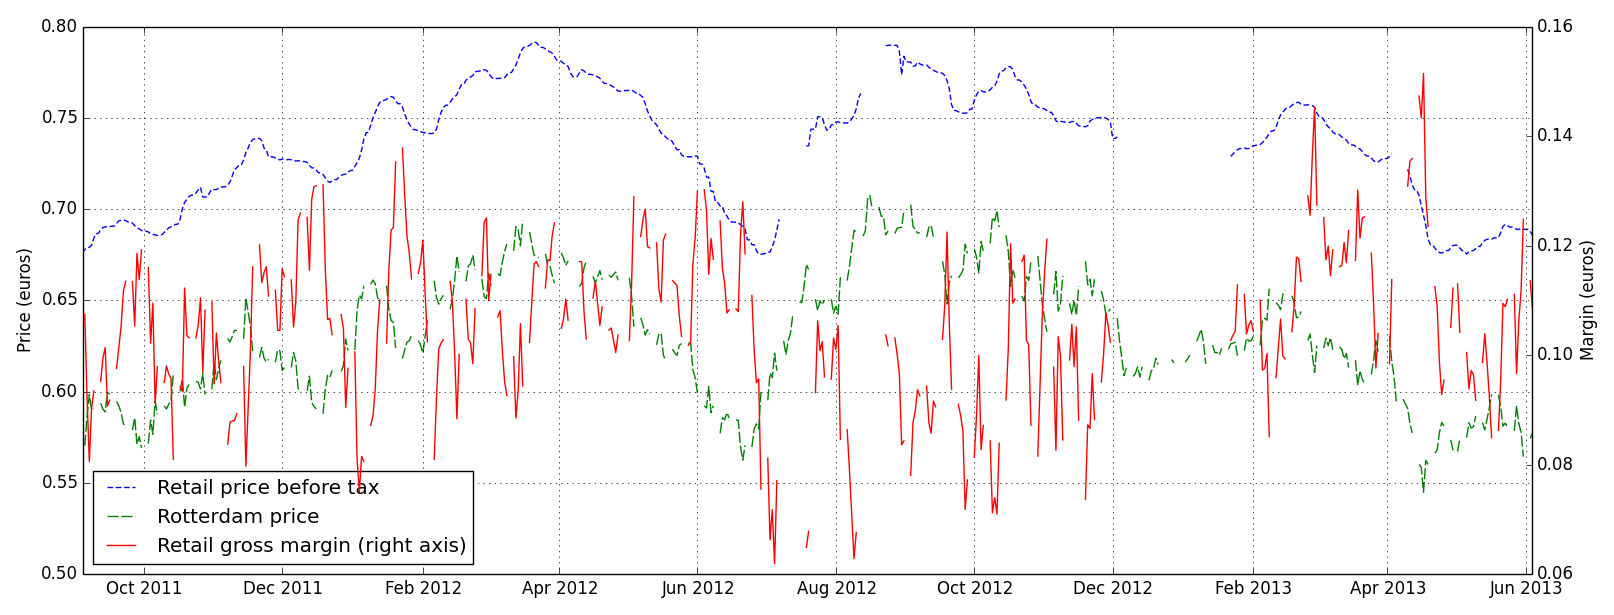
\includegraphics[width=16cm]{graphs/diesel_price_margin.png}
\end{figure}

\textbf{Price ridigity}

Data include prices at 9,932 gas stations in Mainland France, of which 421 are identified as highway gas stations and thus excluded from the analysis. Additionnally, 381 stations are excluded due to apparent poor data quality (less than 10 prices observed or less than a price change per month). Overall, the number of prices observed varies between 8,715 and 8,965 across days in the period studied. On average, XXX gas stations (c. XXX\% of gas stations recorded on the website) change prices within a day. On average, a gas station changes its price every XXX days.

\begin{figure}[!h]
    \caption{Daily number of price changes (09/2011-06/2012)}
	\centering
		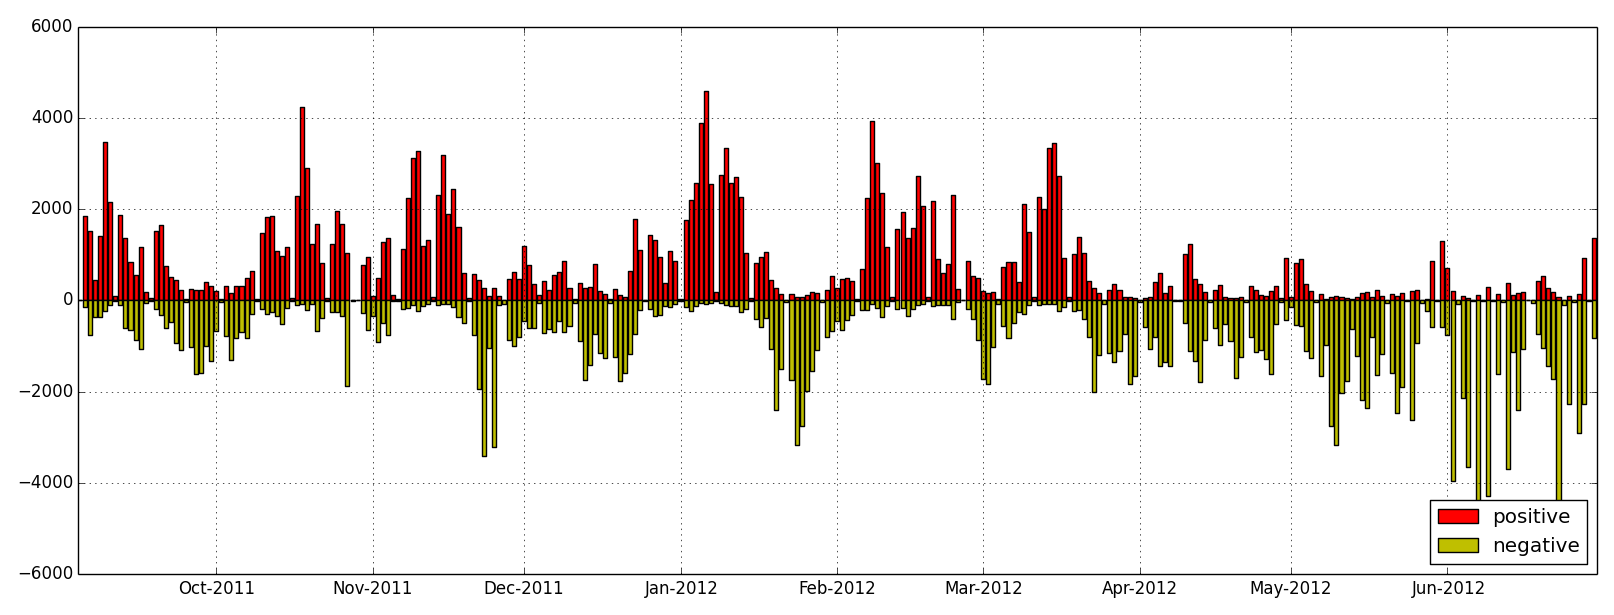
\includegraphics[width=16cm]{graphs/diesel_nb_price_chges.png}
    \floatfoot{The daily collection of prices has occasionally been delayed by a few hours resulting in some imprecision regarding the exact number of price changes occurring within one day}
\end{figure}


\textbf{Heterogeneity among gas stations}

Static price dispersion in French Data is easily seen in any single day price cross section. The resulting price distribution is bimodal, largely reflecting the presence of two dominant types of actors: supermarkets and oil companies. Supermarkets typically state that they use gasoline to attract consumers, while oil companies mention the quality of the service to justify higher prices. Oil companies also traditionally enjoy more demand from businesses with which they develop exclusive relationships in exchange for consumption tracking tools (firm employees pay with a specific magnetic card) and rebates. Price displayed at the gas station is then irrelevant to the transaction.

In comparison, data used in \cite{TAP11} include prices of gas (regular, mid-grade, premium) and diesel at gas stations in California, Florida, Texas and New Jersey from January 2006 to May 2007. The average price of regular gas fluctuates quite a bit over time (from c.\$2.5/gal to c.\$3.5/gal for California) and from one state to the other (average price in Texas over all stations and periods is \$2.576/gal vs. \$3.019/gal in California), largely due to difference in taxes. The number of rivals within 2 miles (c.3.2km) of each station is rather similar in all states: from 13.38 in New Jersey to 14.22 in Texas (resp. 4.25 to 4.74 with 1 mile). The average distance to the closest rival ranges from 0.38 to 0.49 miles (c. 600 to 800m).

\section{Consumer search vs. price levels and dispersion}

Though any attempt to evaluate the degree of consumer information directly through statistics compiled from all potential sources appears futile, Zagaz.com and Prix-carburant.gouv.fr offer the opportunity to observe trend in user registrations and/or trafic. Such information can then be merged with price data to study the relation between proxies for consumer search efforts and price levels or dispersion.

\section{Price dispersion vs. consumer information}

A simple way to measure temporal price dispersion between two stations with daily observations is to consider the probability that the station which is in general cheaper (in terms of day count) turns out to be more expensive. Formally, considering the prices $p_{it}$ and $p_{jt}$ of two stations $i$ and $j$ over $T_{ij}$ days, such that $p_{it} >= p_{ij}$ is observed most of the time, the rank reversals statistic writes:

\begin{align*}
r_{ij} = \frac{1}{T_{ij}} \sum_{t=1}^{T_{ij}} \mathbbm{1}_{p_{jt} > p_{it}}
\end{align*}

Though the computation and intuition of rank reversals is fairly straightforward, its actual use involves dealing with two fundamental practical questions. Though rank reversals at nearby competitors certainly provide more convincing evidence of temporal price dispersion linked to consumer information than variations in the distribution of prices at a municipal/regional/national level, it raises the issue of actual market definition. Also, as static price dispersion leads to a reduction in temporal price dispersion ceteris paribus (in the case of randomization over utilities, there may be dispersion without rank reversals at all), one may need to control for it. As the issue of static price dispersion gets more severe, it can become unclear to which extent nearby sellers actually compete for the same customers, potentially connecting the two questions.

\begin{figure}[H]
\centering
\begin{subfigure}{.4\linewidth}
\centering
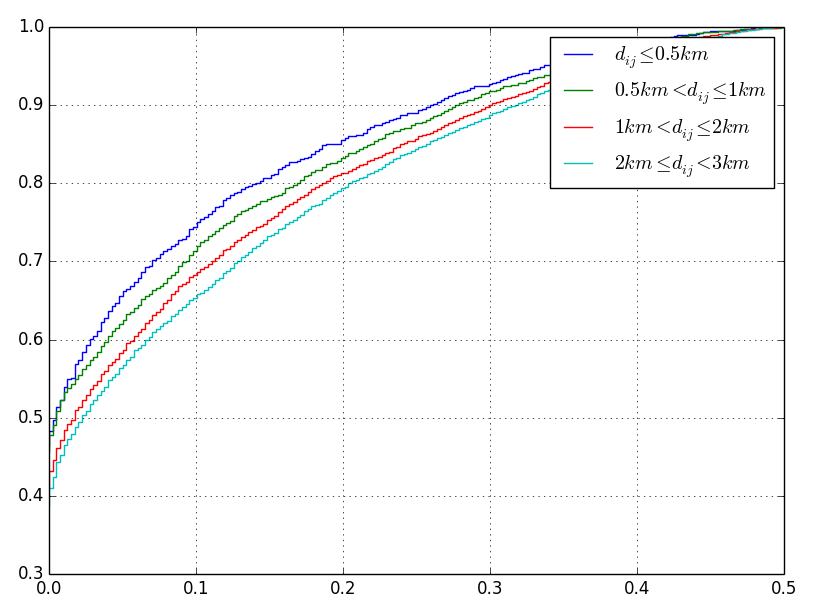
\includegraphics[width=6cm]{graphs/ecdf_rr_all.png}
\caption[short]{All pairs}
\end{subfigure}
\begin{subfigure}{.4\linewidth}
\centering
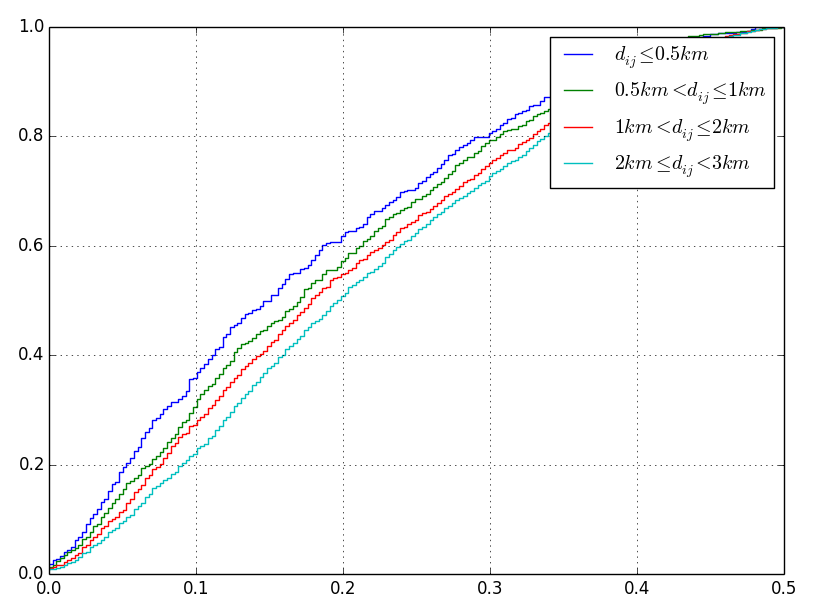
\includegraphics[width=6cm]{graphs/ecdf_rr_nodiff.png}
\caption[short]{Pairs with low differentiation}
\end{subfigure}
\end{figure}

Statistics provided in \cite{TAP11} to describe prices and mark up suggest that the issue of static price dispersion is not severe. In all pairs obtained with a 1 mile maximum distance between stations, depending on fuel type, average spread amounts to 1\% to 2\% of average price, over 90\% of pairs exhibit positive rank reversals, and the average pair rank reversals varies between c.12\% and c.15\%. Results do not vary significantly with a 2 mile maximum distance. Static price dispersion can therefore arguably be neglected, thus avoiding the shortcomings associated with price cleaning.

Using maximum 1km and 2km allows to build databases containing respectively X and X pairs of gas stations. As expected, rank reversals between two stations decreases in the average spread between their prices, with a large number exhibiting no rank reversals. In order to reduce the influence of static dispersion, the sample is subset based on the value of the average spread between prices. Results are presented for a maximum average spread of 0.02c/l i.e. a 1\% to 2\% average difference in prices (NB: X\% of stations include 3 digits in price display). Finally, a last element is taken in consideration: the conversion of XXX gas stations by the brand Total to low cost gas stations, which generates a large number of spurious rank reversals.

INSERT GRAPHS + STATS DES

The percentage of reversed pairs per day varies between X and X etc.

TODO: test with distance vs. rank reversals (control for spread) considering cleaned prices (compare to Lach and Hosken (relevant?) and raw prices... Noise? + Discuss duration of rank reversals and deterministic moves. Insist on economic significance. (+ dispersion vs. price rigidity?)

\section{Market price dispersion}

While the emphasis has so far been laid on examining empirical evidence about the link between price dispersion and consumer information, the following section seeks to compare predictions from a model a la \cite{VAR80} with French retail gasoline market data.

The methodology employed by \cite{TAP11} consists in considering each gas station successively as the center of a market delimited by a circle of a given radius (robustness of results to variations in radius size is checked). Various statistics accounting for price dispersion can then be computed for each market and period. If one observes $N$ stations close to each other (e.g. with a limit radius of 2km: if no two stations are separated by a distance of more than 2 km) and with prices posted over $T$ periods, this will result in $N*T$ observations as each station is successively considered and, for each station, a statistic representing price dispersion is computed at each period. An expected consequence is that it tends to over represent markets with higher gas station density (typically cities).

Regressions are then run using raw prices and cleaned prices. Also, in order to address the issue of overlapping markets, regression are performed on dispersion data generated in a way that prevents market overlap (the precise metholody is not given?). Descriptive statistics performed on raw prices are provided.

Standard market dispersion statistics such as range and standard deviation are strongly influenced by static price dispersion. As a consequence, contrarily to the previous section where descriptives statistics performed on raw prices arguably provided a most conservative first idea of price dispersion, clean prices are now to be preferred despite their shortcomings. Results are reported with clean prices, raw prices for markets obtained with radiuses of respectively 3 and 5km. Additionnally, results are reported for non overlapping markets built in a way that is detailed in appendix.

\ \\
\begin{figure}
\caption{Overview of market price dispersion}
% {\renewcommand{\arraystretch}{0.8}
\begin{center}
\begin{tabular}{lrrr}
\hline
{} & Radius 5km & Radius 3km & No overlap\\
\hline
Nb of markets & 6794 & 5614 & 386 \\
Avg nb competitors & 11.2 & 6.7 & 3.9 \\
\hline
Raw prices & & & \\
\hline
Market price range & 0.116 & 0.105 & 0.089\\
Market gain from search & 0.046 & 0.044 & 0.036 \\
Market price std & 0.046 & 0.045 & 0.045 \\
\hline
Clean prices & & & \\
\hline
Market price range & 0.033  & 0.028 & 0.020 \\
Market gain from search & 0.017 & 0.014 & 0.010 \\
Market price std & 0.011 & 0.011 & 0.010 \\
\hline
\multicolumn{4}{p{.8\textwidth}}{Each price dispersion statistic corresponds to the average across markets of average price dispersion over time. Markets with less than 3 competitors are dropped. At the market level, price dispersion has been computed only for days when more than two thirds of competitors' prices are available. Only markets with more than 50 days of data are then kept for the overall average.}
\end{tabular}
\end{center}
\end{figure}

\newpage

\bibliography{references}

\newpage

\appendix

\section{Data processing}

Price and station information: Duplicate detection. Not trivial: typically occurs when brand changes... new record with new address/brand... use price information
Investigation of brand changes more detailed in descriptive statistics.

Location: same corner gas station... crucial for consumer information / advantage in location
Duplicates: picture of competition, potentially interesting if stations closed can be found in data.
Brand changes: Connected to duplicates... important policy implications
Highway gas stations: different market

The database which lies behind the website is first essentially recreated, using the same gas station identification numbers as it is contained in webpages (zip code + 3 digits which appear to merely reflect the registration order of gas stations with the same zip code). Two observations follow: there appears to be a significant turnover in the data, some prices appear to reflect mistakes by managers (extraordinary variations in price).

Since there are very few gas stations which are newly opened each year, it must be that gas stations either stop providing information because they are not/no more committed to do so or create a new account and are then registered under a different identification number... hence the need to reconcile them.

Treatment of prices:
\begin{itemize}
\item Daily files are merged recursively on station ids which leads to create a database of 10,433 individuals over 640 days, including unobserved periods which result in missing values within series. Since dates of price changes are known, missing periods can yet be filled in many cases (e.g: if price on day 2 if missing, it can be checked in day 3 that price hasn't changed since day 1 and if price on days 10-15 are missing, it can be seen on day 16 that the last changed was made on day 13: prices for 13-15 are then input backward and forward for 10-12). TODO: stats
\item Abnormal values are then looked for based on prior observation. This allows to observe that some prices are input as 0.156 instead of 1.56 and correct rather than transform in missing values. TODO: stats
\item Abnormal price variations are then looked for based on observation. Quite often it appears that the variation must have been the consequence of a mistake given the size and the following reverse change. Such changes are eliminated. When no converse changes can be found due to missing data, suspect periods are also switched to missing.
\item Abnormal price durations are finally examined based on prior observation. As mentioned in XXX, a duration of 1 month is considered suspect, 1 month and 1/2 highly suspect, 2 months almost certainly an error.
\end{itemize}

Station information:
\begin{itemize}
\item Matching of stations with INSEE codes: Zip codes: problem of cedex and changing zip codes. City name matching implies the generic problem of string comparison, not to mention the fact that the same name can be used in different regions and that city names sometimes change (small municipalities are regrouped). Approach: matching on zip then city name
\item Matching of databases: address standardization but still remains a big issues as quite different addresses can be provided, a piece of info can be up to date in one database while a bit old in the other. It requires a multicriteria approach.
\item Geocoding: address standardization
\item Highway gas stations
\end{itemize}

\end{document}
